\documentclass[dvipdfmx]{jarticle}
\pagestyle{empty}
\hoffset=-25mm \voffset=-25mm
\setlength{\textwidth}{16cm}
\setlength{\textheight}{24cm}
\usepackage{url}
\usepackage{tikz}
\usetikzlibrary{calc,shapes}
\usepackage{fancyvrb}
\usepackage{tabularx}
\usepackage{multirow}
\newcounter{coffee}
\newcounter{bean}
\newcommand{\ttdo}{\texttt{do}}
\newcommand{\ttwhile}{\texttt{while}}
\newcommand{\ttlp}{\texttt{(}}
\newcommand{\ttrp}{\texttt{)}}
\newcommand{\ttsc}{\texttt{;}}
\newcommand{\tteq}{\texttt{=}}
\newcommand{\ttif}{\texttt{if}}
\newcommand{\ttelse}{\texttt{else}}
\newcommand{\ttand}{\texttt{\&\&}}
\newcommand{\ttlt}{\texttt{<}}
\newcommand{\ttsub}{\texttt{-}}

\newcommand{\newLabel}[1]{\texttt{newLabel}({#1})}
\newcommand{\newTemp}[1]{\texttt{newTemp}({#1})}

\newcommand{\makenewtemp}{{\tt newTemp()}}
\newcommand{\makenewlabel}{{\tt newLabel()}}
\newcommand{\gengoto}[1]{{\tt generate(`goto }{#1}{\tt ')}}
\newcommand{\genlabel}[1]{{\tt generate(`label }{#1}{\tt ')}}
\newcommand{\genifnot}[2]{{\tt generate(`if\_not}\ {#1}\ {\tt goto}\ {#2}\ {\tt ')}}
\newcommand{\genassign}[2]{{\tt generate(`}{#1}{\tt :=}{#2}{\tt ')}}

\newcommand{\redtext}[1]{{\color{red}{#1}}}
\begin{document}
\begin{flushright}
\verb|2026/10/30|
\end{flushright}
\begin{center}{\bf\Large
  2026年度　コンパイラ演習課題(5)
}\end{center}
\begin{itemize}
  \item TACTの課題の添付ファイルとしてPDFファイルで提出すること．
  \item 手書きレポートをPDFとして提出方法は講義webサイトを
  参照\footnote{\url{https://sites.google.com/sqlab.jp/26compiler/how-to-make-report}}すること．
  \item 提出期限: 11月6日(金) 23:55(JST)
\end{itemize}

\begin{list}{{\bf [\,\arabic{coffee}\,]}}{\usecounter{coffee}}
 \item フィボナッチ関数のプログラムを以下のように与える．

       \begin{Verbatim}[frame=single]
int a;
fib(int x) {
  if ( x <= 0 ) return(0);
  else if ( x==1 ) return(1);
  else return(fib(x-2)+fib(x-1));
}

main() {
  a = 3;
  printf("%d\n",fib(a));
}
       \end{Verbatim}

       \verb|fib|と\verb|return|の実行と駆動レコードの様子を図式化せよ．
       講義スライドと同様のレベルで図式化すること．

\item 次のCF文法$G_1$について答えよ．

$G_1=\langle\{S,C,D,E\},\{\ttdo,\ttwhile,\ttlp,\ttrp,\ttsc,\tteq,\ttif,\ttelse,\ttand,\ttlt,\ttsub,\mathsf{id}\},P,S\rangle$
\[P=\left\{\begin{array}{llllll}
  1: & S\rightarrow\ttdo\ S^{(1)}\ \ttwhile\ \ttlp\ E\ \ttrp\ttsc &
  4: & E\rightarrow E^{(1)}\ttand D & 7: & D\rightarrow C\\
  2: & S\rightarrow\mathsf{id}\tteq E & 5: & E\rightarrow D & 8: & C\rightarrow C^{(1)}\ttsub\mathsf{id}\\
  3: & S\rightarrow\ttif\ttlp E\ttrp\ S^{(1)}\ \ttelse\ S^{(2)} &
  6: & D\rightarrow D^{(1)}\ttlt C & 9: & C\rightarrow\mathsf{id}
\end{array}\right\}\]

\begin{list}{(\alph{bean})}{\usecounter{bean}}
  \item 規則1のコード生成ルーチンを与えよ．
  \[S\rightarrow\ttdo\{\fbox{\mbox{\quad (1)\quad}}\}\;S^{(1)}\ttwhile\ttlp E\ttrp\ttsc
  \{\fbox{\quad (2)\quad}\}\]

  \item その他の規則に対する生成ルーチンは以下のようになる．
  (裏面へ続く)
  \begin{center}
    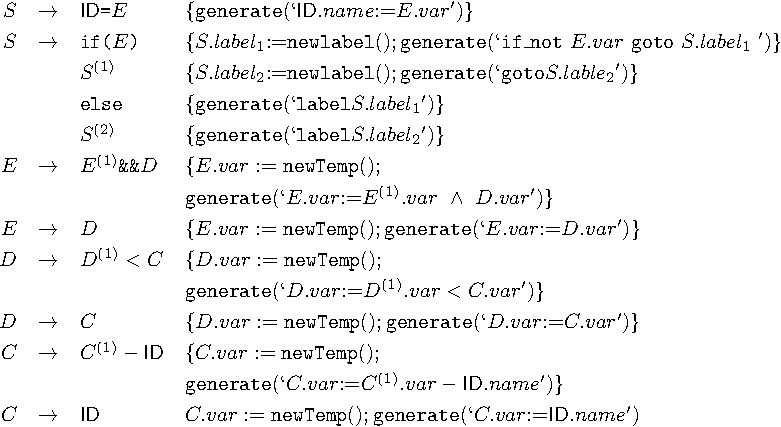
\includegraphics{semantic-rules1-crop.pdf}
  \end{center}

  $\ttdo\ \ttif\ \ttlp\texttt{x1}\ttlt\texttt{x2}\ttrp\ \texttt{x1=x1-x3}\ \ttelse\ \texttt{x2=x2-x4}\ \ttwhile
  \ttlp\texttt{x5<x1-x6}\ \ttand\ \texttt{x7<x1}\ttrp\ttsc$

  から生成される３番地コードのプログラムを示せ．
\end{list}
\end{list}

\end{document}